\documentclass[12pt]{article}

\usepackage{url}
\usepackage{color}
\usepackage{float}
\usepackage{array}
\usepackage{xcolor}
\usepackage{multirow}
\usepackage{graphicx}
\usepackage{booktabs}
\usepackage{colortbl}
\usepackage{hyperref}
\usepackage{spreadtab}
\usepackage{longtable}
\usepackage{pdflscape}
\usepackage[T1]{fontenc}
\usepackage[utf8]{inputenc}
\usepackage[english]{babel}
\usepackage[margin=1.5cm]{geometry}
\usepackage[format=hang,labelfont=bf,font=small]{caption}
\usepackage{mathtools, amsmath, amsthm, amssymb, amsfonts, mathpartir}

\begin{document}

\title{Deep Learning: Homework 1}
\author{Hugo Mantinhas 95592, João Silveira 95597}

\maketitle

\section*{Work Division}

Each member of the group worked together on all the questions in this assignment. For this reason, the workload was divided equally between the two members of the group.

\section*{Question 1}
\begin{itemize}
    \item \textbf{1. a)}
          \begin{table}[H]
              \centering
              \begin{tabular}{|c|c|c|c|}
                  \toprule
                                    & \textbf{Train} & \textbf{Validation} & \textbf{Test} \\
                  \midrule
                  \textbf{Accuracy} & 0.4654         & 0.4610              & 0.3422        \\
                  \bottomrule
              \end{tabular}
              \label{tab:1.1a}
              \caption{Train, validation and test accuracies for the perceptron model}
          \end{table}

          \begin{figure}[H]
              \centering
              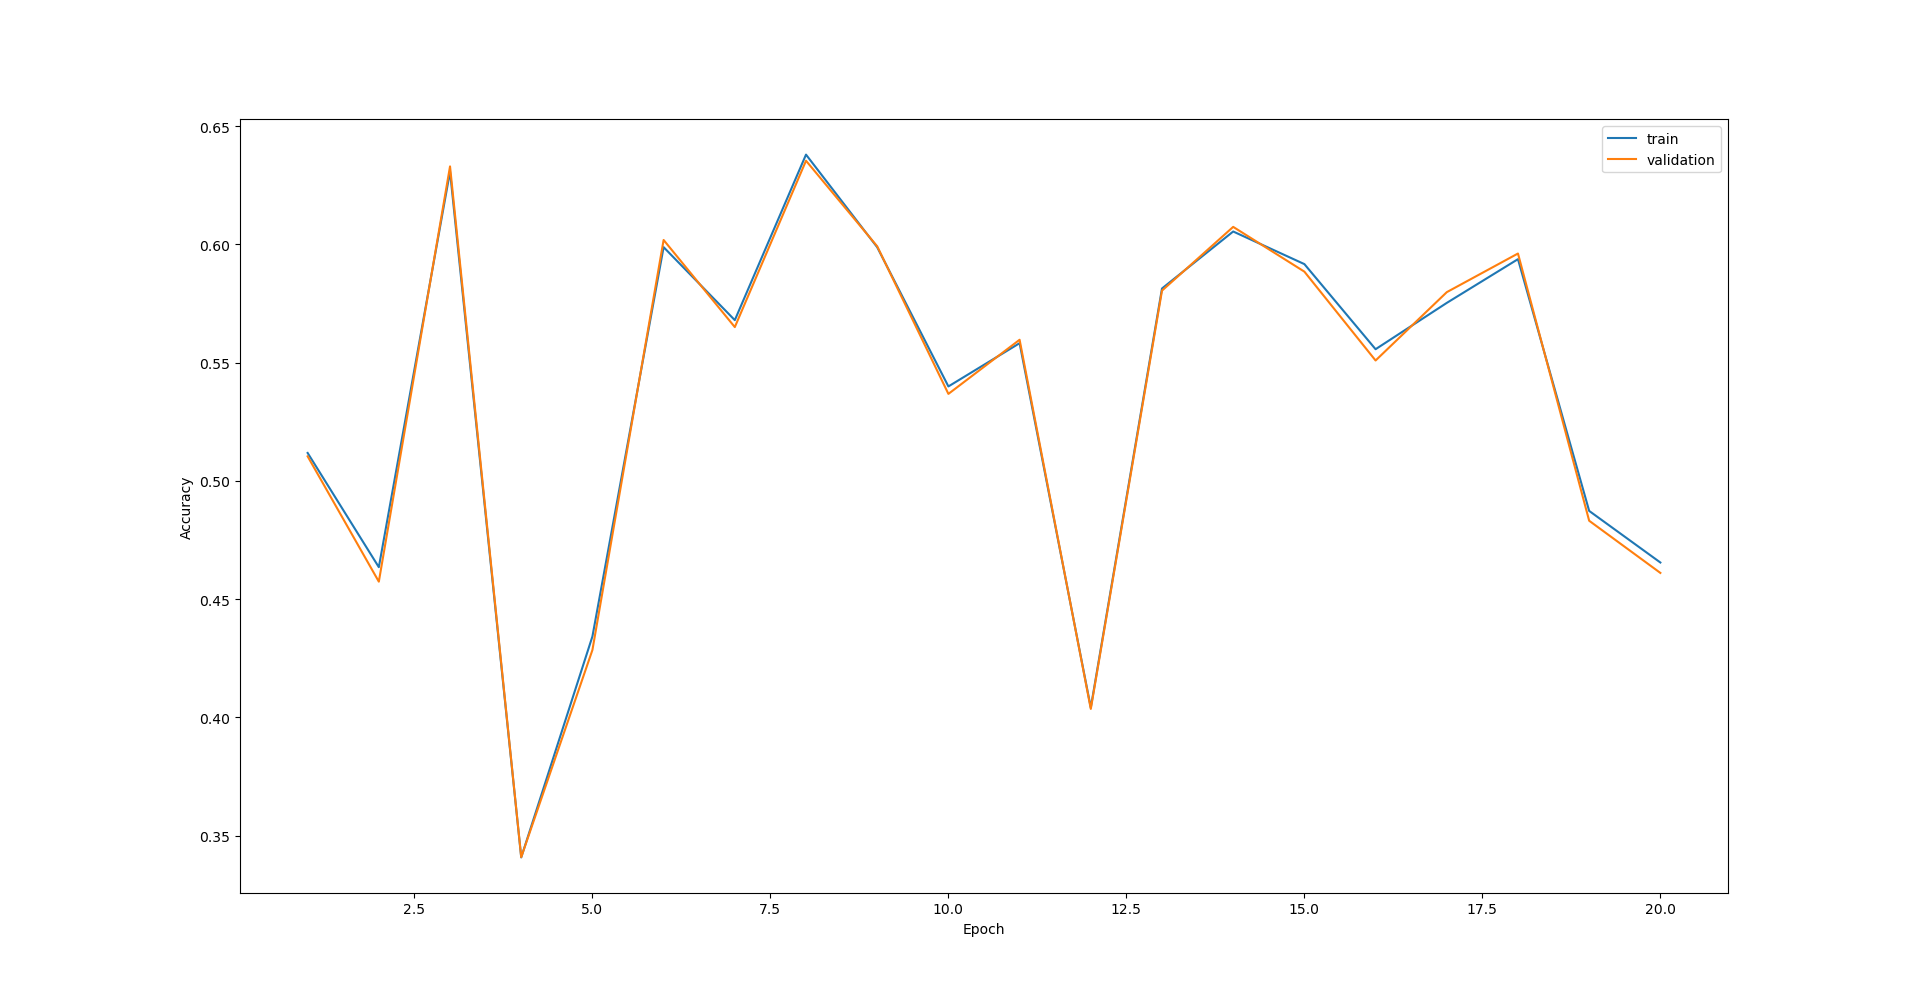
\includegraphics[width=1\linewidth]{../outputs/hw1-q1-1a.png}
              \caption{Train and validation accuracies as a function of the number of epochs for the perceptron model}
              \label{fig:1.1a}
          \end{figure}
          \clearpage

    \item \textbf{1. b)} Analyzing the plot for the learning rate of 0.01, we find that the weight update many times results in accuracy changes in the order of 5\%, in both directions. This suggests that the weight adjustments might be overshooting the optimal value. On the other hand, the learning rate of 0.001 results in a more stable learning process, with the accuracy changes being in the order of 1\% or less. Unlike the model trained with 0.01 learning rate, this one seems to be tending to grow over time which suggests that the weight adjustments are closer to the optimal value. Although the final test accuracies for both models don't look much different: 0.5784 for learning rate 0.01 and 0.5936 for learning rate 0.001; for the latter the model shows a lot more stability in its accuracy across epochs.
          \begin{figure}[H]
              \centering
              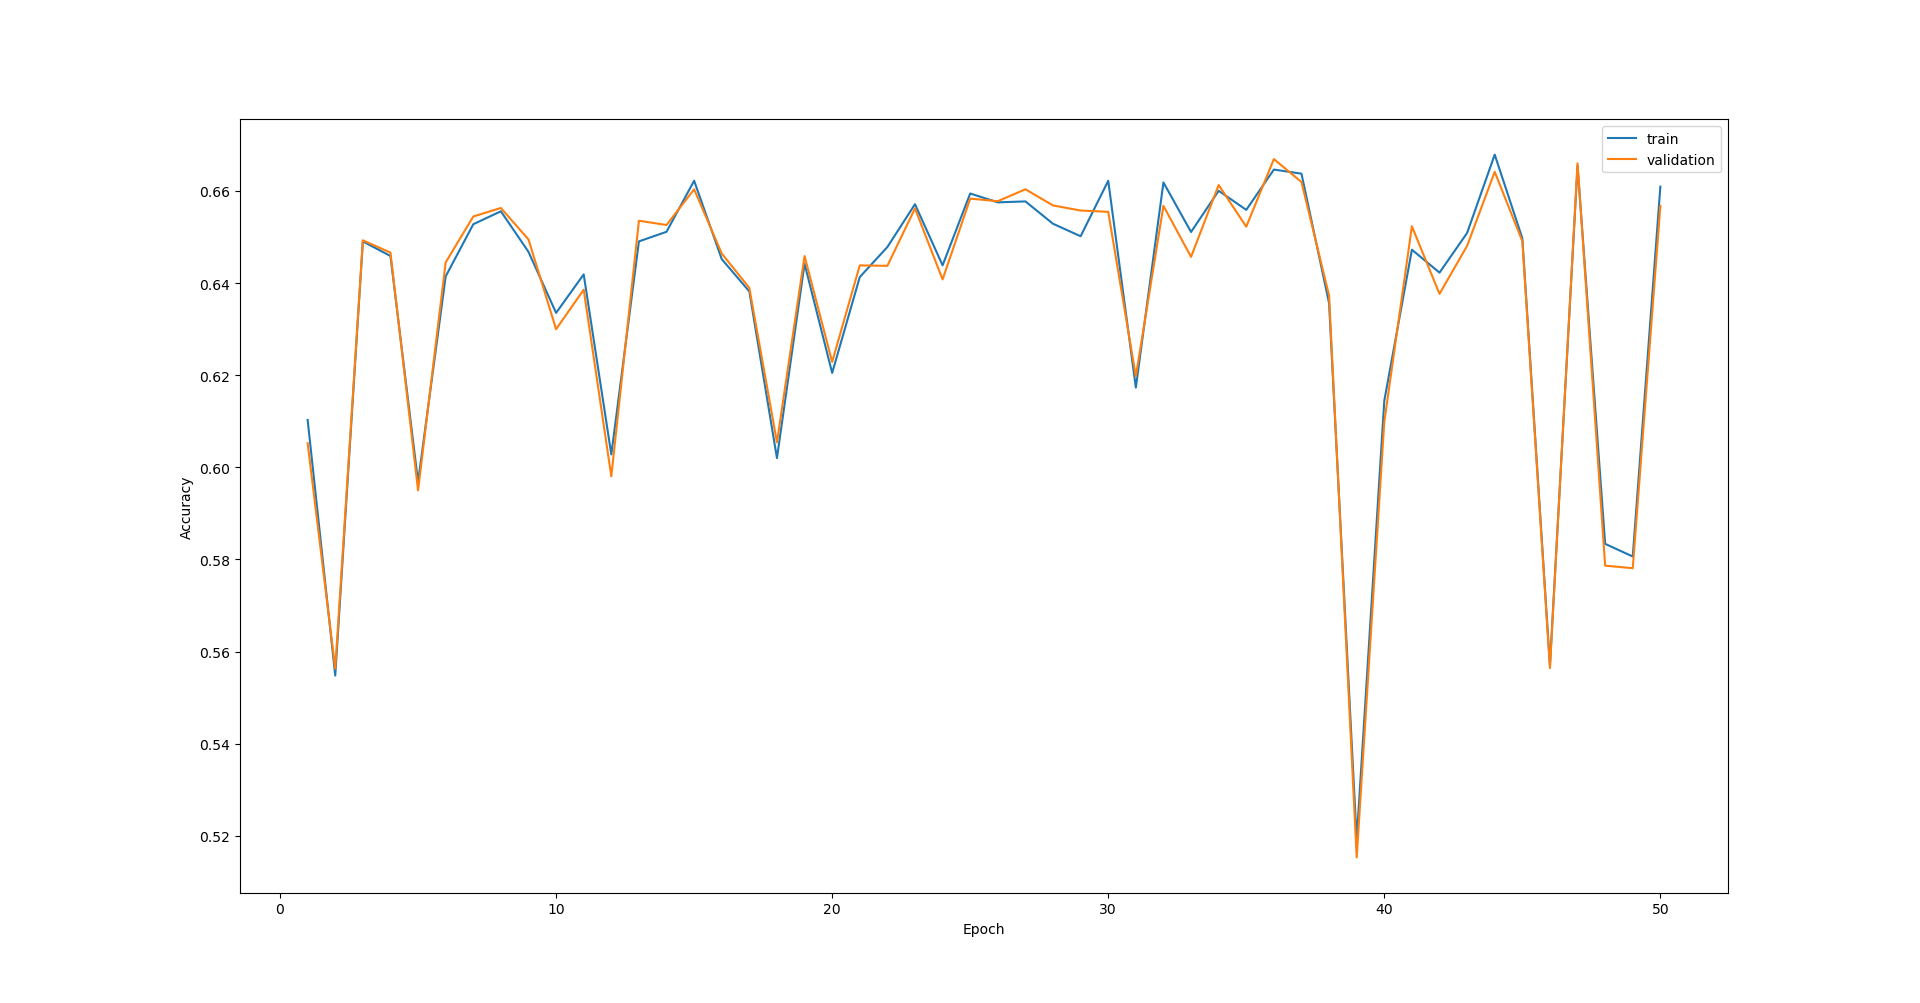
\includegraphics[width=1\linewidth]{../outputs/hw1-q1-1b.01.png}
              \caption{Train and validation accuracies as a function of the number of epochs for learning rate of 0.01}
              \label{fig:1.1b:0.01}
          \end{figure}

          \begin{figure}[H]
              \centering
              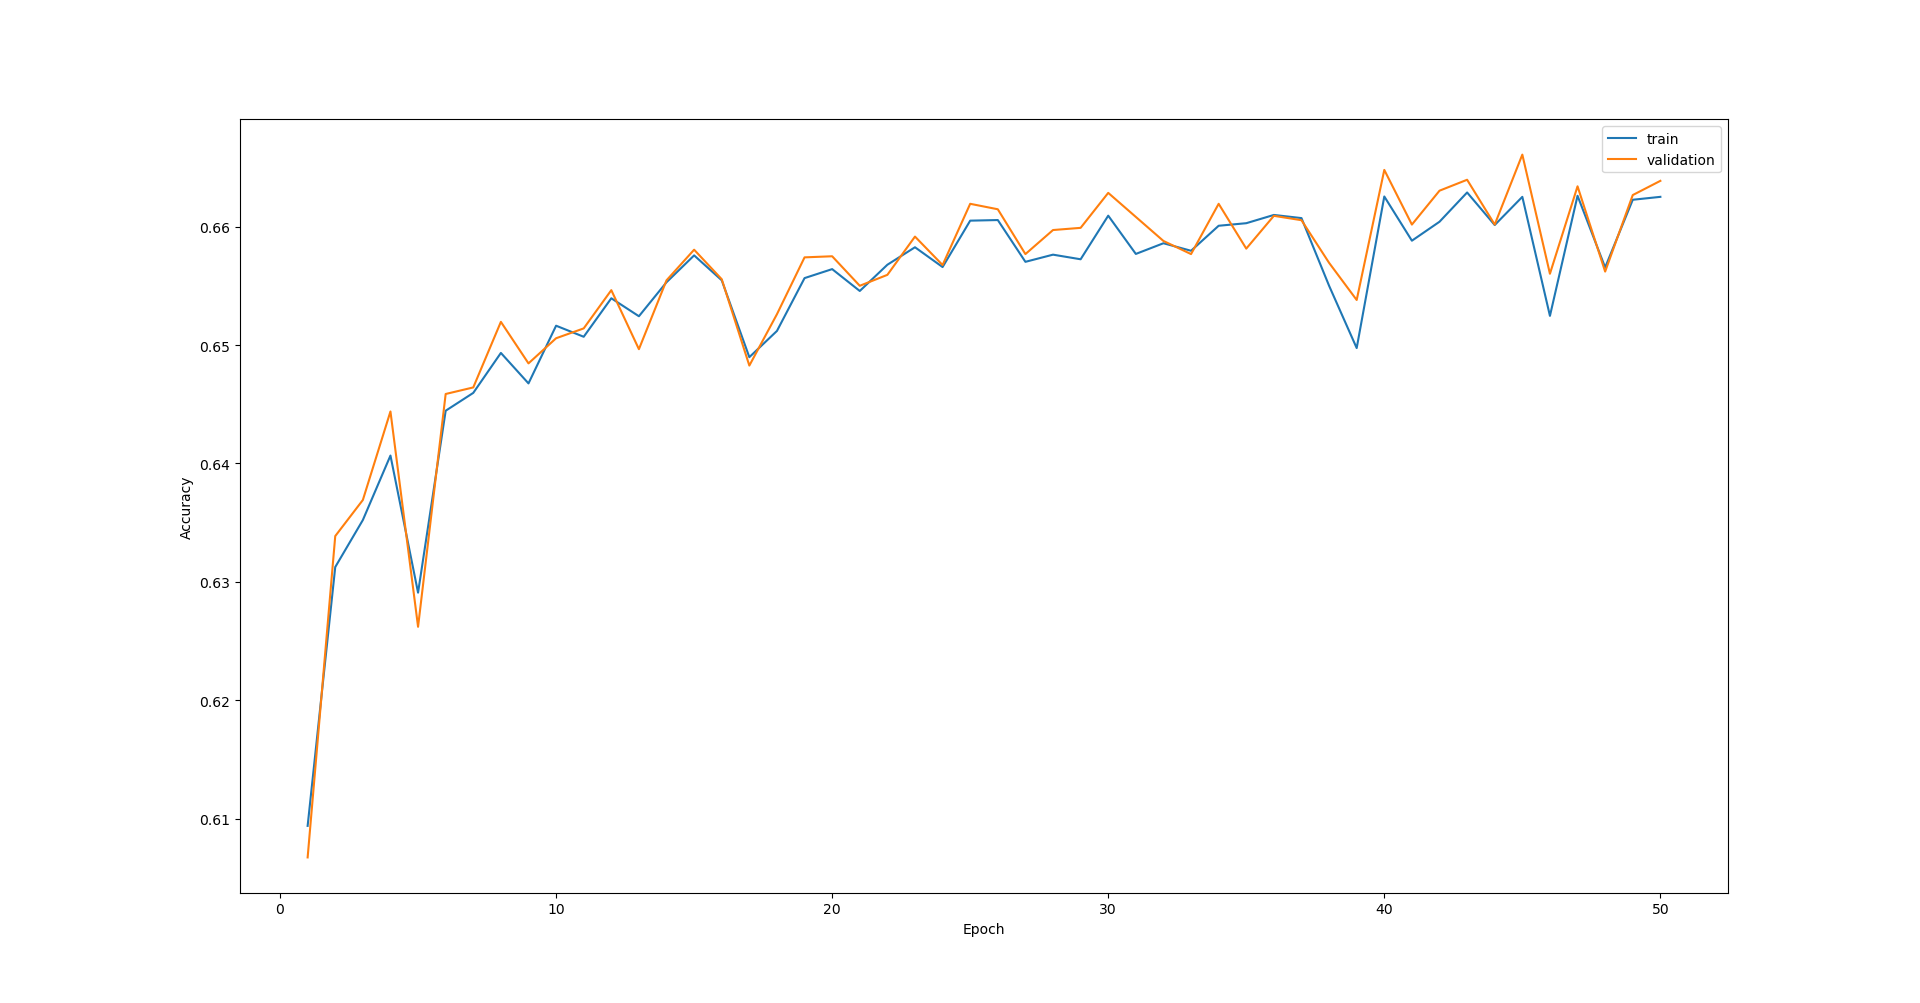
\includegraphics[width=1\linewidth]{../outputs/hw1-q1-1b.001.png}
              \caption{Train and validation accuracies as a function of the number of epochs for learning rate of 0.001}
              \label{fig:1.1b:0.001}
          \end{figure}

          \begin{table}[H]
              \centering
              \begin{tabular}{|c|c|c|c|}
                  \toprule
                                               & \textbf{Train} & \textbf{Validation} & \textbf{Test} \\
                  \midrule
                  \textbf{Learning rate 0.01}  & 0.6609         & 0.6568              & 0.5784        \\
                  \textbf{Learning rate 0.001} & 0.6625         & 0.6639              & 0.5936        \\
                  \bottomrule
              \end{tabular}
              \label{tab:1.1b}
              \caption{Train, validation and test accuracies for learning rates of 0.01 and 0.001}
          \end{table}

    \item \textbf{2. a)} This statement is true. A logistic regression model is a linear model, which means that it can only learn linearly separable data, i.e., a dataset whose classes can be separated by a hyperplane. On the other hand, a multi-layer perceptron using \texttt{relu} activations can learn to separate non-linearly separable data because of the non-linearity introduced by the \texttt{relu} activation function in between layers. However, it can be shown, by computing the Hessian matrix of the loss function, that the loss function of a logistic regression model using cross-entropy loss is always convex. However, the same cannot be done for the loss function of a multi-layer perceptron, in general. This means that the logistic regression model can be trained to a global optimum, while, when using a multi-layer perceptron, we can never be sure that we have reached a global optimum.

    \item \textbf{2. b)} The final test accuracy is 0.7580.
          \begin{figure}[H]
              \centering
              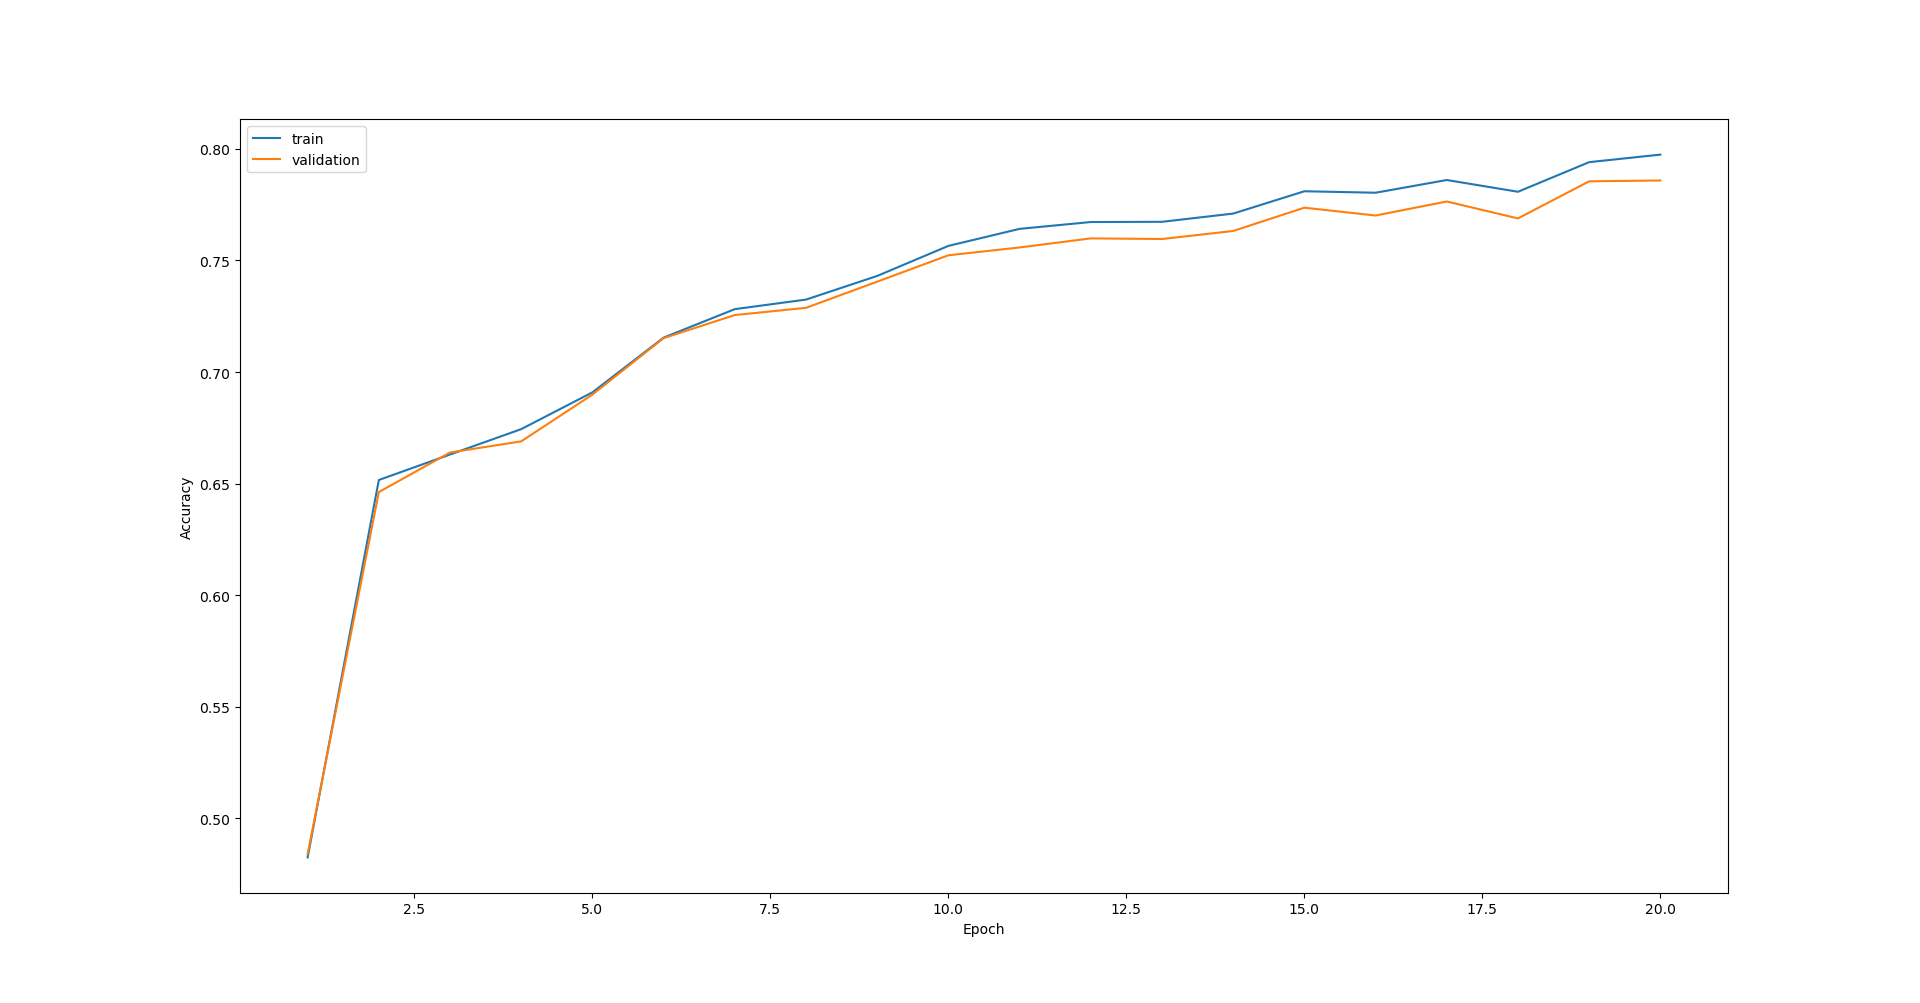
\includegraphics[width=1\linewidth]{../outputs/hw1-q1-2b.001-acc.png}
              \caption{Train and validation accuracies as a function of the number of epochs for the no-toolkit MLP}
              \label{fig:1.2b:acc}
          \end{figure}

          \begin{figure}[H]
              \centering
              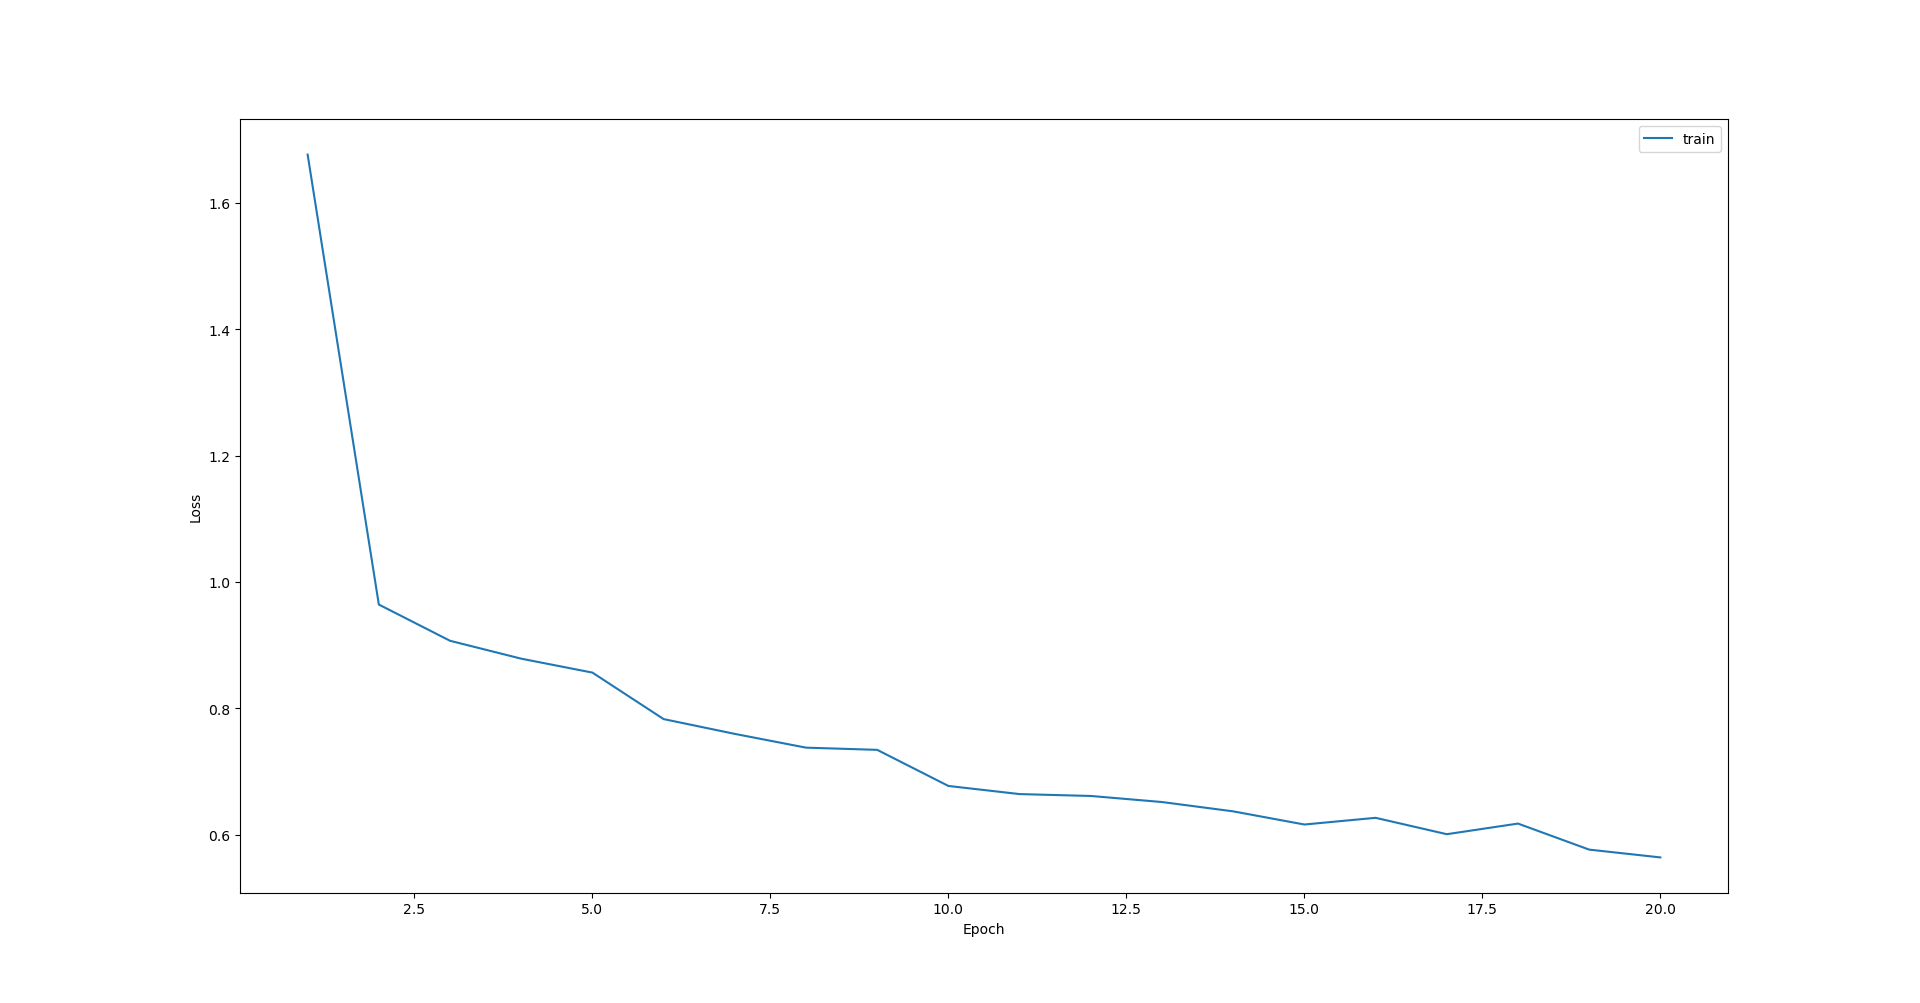
\includegraphics[width=1\linewidth]{../outputs/hw1-q1-2b.001-loss.png}
              \caption{Train loss as a function of the number of epochs for the no-toolkit MLP}
              \label{fig:1.2b:loss}
          \end{figure}
\end{itemize}

\section*{Question 2}
\begin{itemize}
    \item \textbf{1.} The best configuration in terms of validation accuracy was the one with learning rate 0.01, with a validation accuracy of 0.6535. Its final test accuracy is 0.6200.
          \begin{figure}[H]
              \centering
              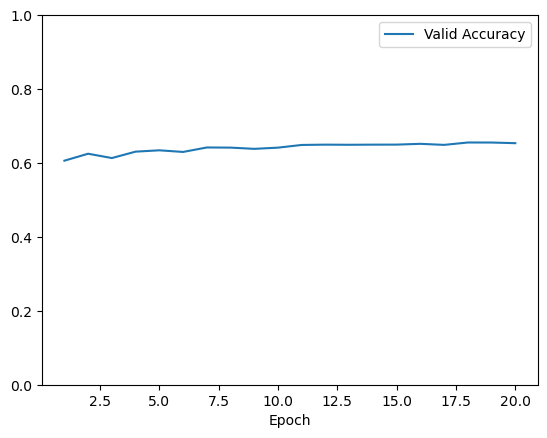
\includegraphics[width=0.5\linewidth]{../outputs/hw1-q2-1-acc.01.png}
              \caption{Validation accuracy as a function of the number of epochs for the logistic regression model with learning rate 0.01}
              \label{fig:2.1:acc}
          \end{figure}

          \begin{figure}[H]
              \centering
              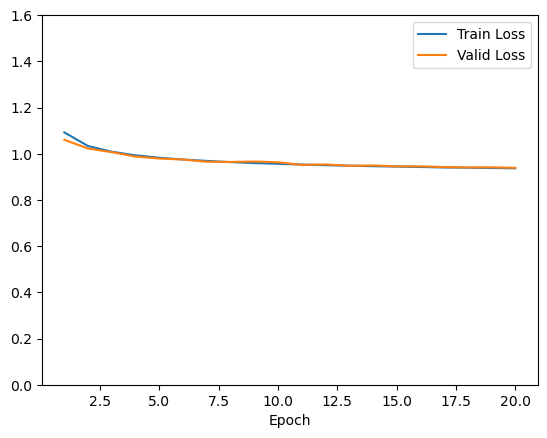
\includegraphics[width=0.5\linewidth]{../outputs/hw1-q2-1-loss.01.png}
              \caption{Train and validation loss as function of the number of epochs for the logistic regression model with learning rate 0.01}
              \label{fig:2.1:loss}
          \end{figure}

    \item \textbf{2. a)}
          The choice of the batch size hyperparameter imposes dealing with a trade-off between test accuracy and training time. Smaller batches produce more frequent gradient updates, but this comes at the cost of making more non-parallelizable computations. Moreover, as we decrease the batch size, the more noisy the gradient signal becomes, which, in the extreme case, causes unstable training. However, when chosen properly, a smaller batch size offers a regularizing effect, since it introduces noise in the gradient signal, which can help the model generalize better. Larger batch sizes, on the other hand, produce less frequent gradient updates, meaning that, in each epoch, we need to do less non-parallelizable computations and, therefore, each epoch takes less time to complete. However, in the extreme case, large batch sizes can lead to overfitting, since the gradient signal is less noisy.

          In this case, we can see that the model with batch size 16 has a better test accuracy than the model with batch size 1024. However, the model with batch size 1024 has a much faster training time, in this case, 3.5 times faster. This is because, in each epoch, the model with batch size 16 needs to perform 64 times more non-parallelizable computations than the model with batch size 1024.

          \begin{table}[H]
              \centering
              \begin{tabular}{|c|cc|}
                  \toprule
                  \textbf{Batch Size} & \textbf{Test Accuracy} & \textbf{Execution time} \\
                  \midrule
                  \textbf{16}         & \underline{0.7788}     & 1min17.420sec           \\
                  \textbf{1024}       & 0.7208                 & 0min22.466sec           \\
                  \bottomrule
              \end{tabular}
              \caption{Test accuracy and execution time for the feed-forward network with batch sizes 16 and 1024}
              \label{tab:2.2a}
          \end{table}

          \begin{figure}[H]
              \centering
              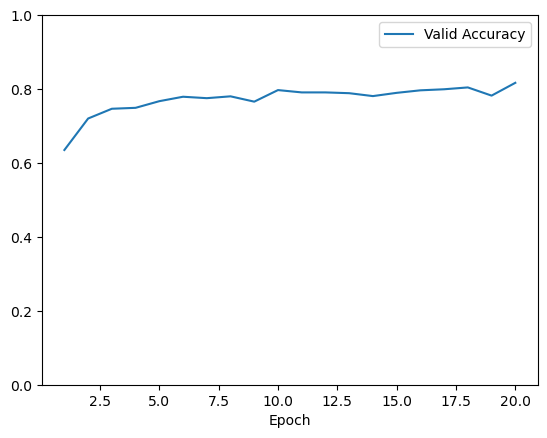
\includegraphics[width=0.5\linewidth]{../outputs/hw1-q2-2a-acc-16.png}
              \caption{Train and validation accuracies as a function of the number of epochs for the feed-forward network using a batch size of 16}
              \label{fig:2.2a:acc:16}
          \end{figure}

          \begin{figure}[H]
              \centering
              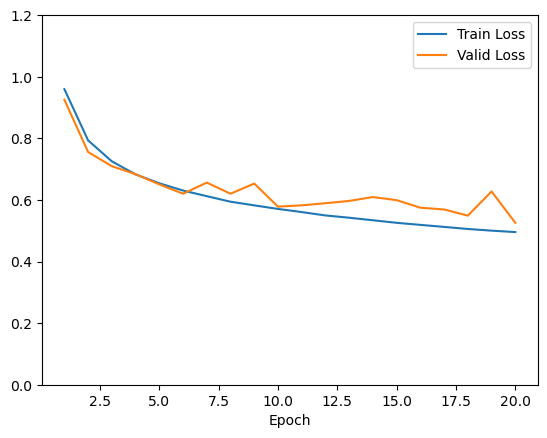
\includegraphics[width=0.5\linewidth]{../outputs/hw1-q2-2a-loss-16.png}
              \caption{Train and validation loss as a function of the number of epochs for the feed-forward network using a batch size of 16}
              \label{fig:2.2a:loss:16}
          \end{figure}

          \begin{figure}[H]
              \centering
              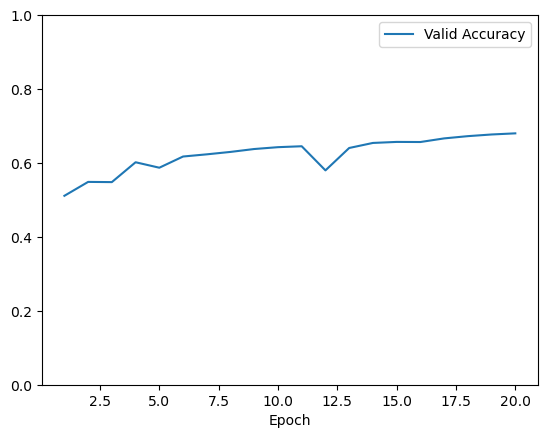
\includegraphics[width=0.5\linewidth]{../outputs/hw1-q2-2a-acc-1024.png}
              \caption{Validation accuracy as a function of the number of epochs for the feed-forward using a batch size of 1024}
              \label{fig:2.2a:acc:1024}
          \end{figure}

          \begin{figure}[H]
              \centering
              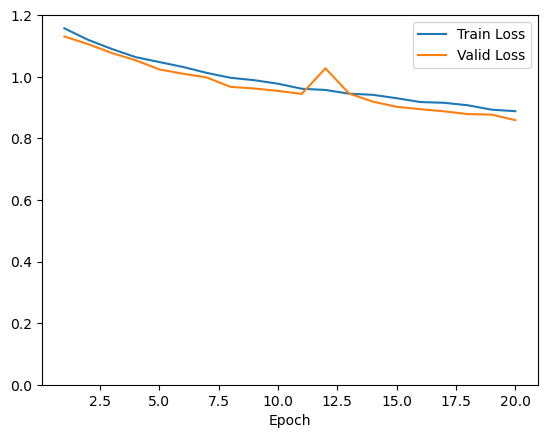
\includegraphics[width=0.5\linewidth]{../outputs/hw1-q2-2a-loss-1024.png}
              \caption{Train and validation loss as a function of the number of epochs for the feed-forward using a batch size of 1024}
              \label{fig:2.2a:loss:1024}
          \end{figure}

    \item \textbf{2. b)} The best and worst configurations in terms of validation accuracy were the ones with learning rates 0.1 and 1, respectively. The best configuration has a validation accuracy of 0.8168 and a test accuracy of 0.7788 which is also the best test accuracy achieved across all configurations. The worst configuration, on the other hand, has a validation accuracy of 0.4721 and a test accuracy of 0.4726. The configuration using a learning rate of 1 is the worst because the model overshoots the optimal gradient descent step, which, in turn, inhibits the model from converging to a good solution. On the other hand, the configuration using a learning rate of 0.1 is the best because it is small enough to allow the model to converge to a good solution, but large enough to allow the model to converge in a reasonable amount of time.
          \begin{figure}[H]
              \centering
              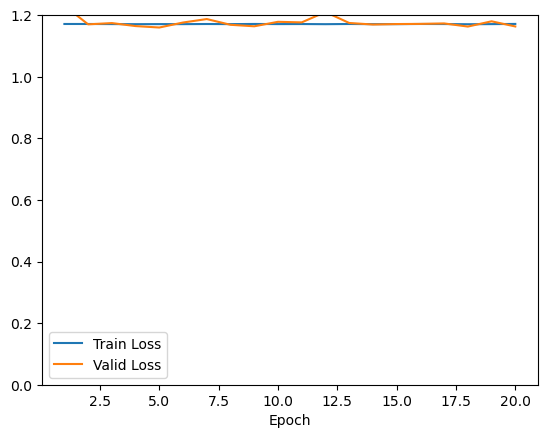
\includegraphics[width=0.5\linewidth]{../outputs/hw1-q2-2b-loss-1.png}
              \caption{Train and validation loss as a function of the number of epochs for the feed-forward network using a learning rate of 1}
              \label{fig:2.2b:acc}
          \end{figure}

          \begin{figure}[H]
              \centering
              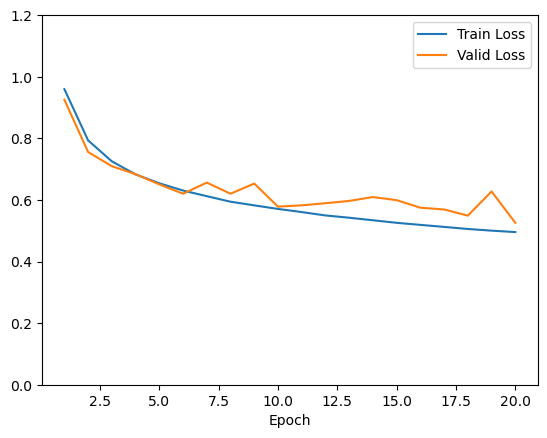
\includegraphics[width=0.5\linewidth]{../outputs/hw1-q2-2b-loss-.1.png}
              \caption{Train and validation loss as a function of the number of epochs for the feed-forward network using a learning rate of 0.1}
              \label{fig:2.2b:loss}
          \end{figure}

    \item \textbf{2. c)} The best and worst configurations in terms of validation accuracy were the one using dropout rates of 0.2 and the one using L2 regularization parameter set to 0.0001, respectively. The best test accuracy was achieved by the configuration using dropout rates of 0.2, with a test accuracy of 0.8034. The default model showed signs of overfitting, since the validation loss stopped improving after around 50 epochs, while the training loss kept improving. This means that the model started to learn the training data too well, which caused it to generalize poorly to the validation data. Using a L2 a regularization parameter of 0.0001 did not help much the model generalize better, since the validation loss stopped improving after around 60 epochs. However, the model using dropout rates of 0.2 was able to generalize better, since the validation loss kept improving until 120 epochs. This improved generalization capability is reflected in the test accuracy achieved by each model, with the model using dropout rates of 0.2 achieving a test accuracy of 0.8034, while the default model and the model using L2 regularization parameter of 0.0001 achieved test accuracies of 0.7750 and 0.7864, respectively.
          \begin{figure}[H]
              \centering
              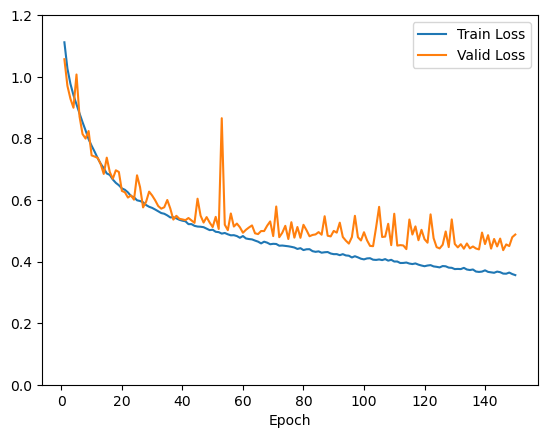
\includegraphics[width=0.5\linewidth]{../outputs/hw1-q2-2c-default-loss.png}
              \caption{Train and validation loss as a function of the number of epochs for the default feed-forward network}
              \label{fig:2.2c:default:loss}
          \end{figure}

          \begin{figure}[H]
              \centering
              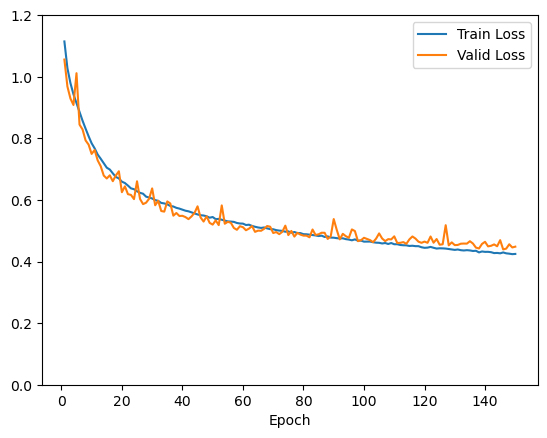
\includegraphics[width=0.5\linewidth]{../outputs/hw1-q2-2c-dropout-loss.png}
              \caption{Train and validation loss as a function of the number of epochs for the feed-forward network using dropout rates of 0.2}
              \label{fig:2.2c:dropout:loss}
          \end{figure}

          \begin{figure}[H]
              \centering
              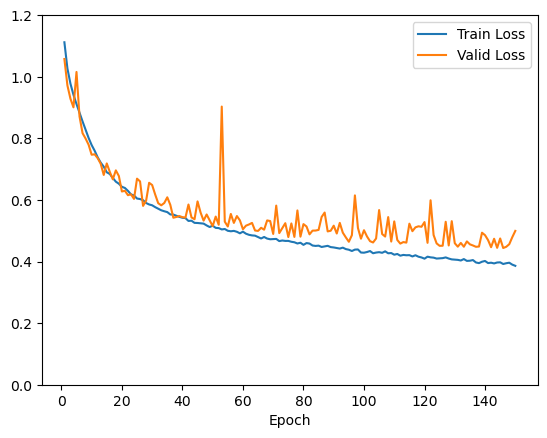
\includegraphics[width=0.5\linewidth]{../outputs/hw1-q2-2c-l2-loss.png}
              \caption{Train and validation loss as a function of the number of epochs for the feed-forward network using L2 regularization parameter set to 0.0001}
              \label{fig:2.2c:l2:loss}
          \end{figure}
\end{itemize}

\section*{Question 3}
\begin{itemize}
    \item \textbf{1. a)} For the case with $D=2, A=-1, B=1$, there are 4 data points in our domain, calculated in Figure \ref{fig:3a:calc}, and represented in Figure \ref{fig:3a:graph}

        \begin{figure}[H]
            \begin{minipage}{0.5\linewidth}
                \begin{equation*}
                    f(-1, 1):
                \end{equation*}
                \begin{equation*}
                    \sum_{i=1}^{2} x_i = -1 + 1 = 0
                \end{equation*}
                \begin{equation*}
                    0 \in [-1, 1] \Rightarrow f(-1, 1) = 1
                \end{equation*}

                \begin{equation*}
                    f(-1, -1):
                \end{equation*}
                \begin{equation*}
                    \sum_{i=1}^{2} x_i = -1 + -1 = -2
                \end{equation*}
                \begin{equation*}
                    -2 \notin [-1, 1] \Rightarrow f(-1, -1) = -1
                \end{equation*}
            \end{minipage}
            \begin{minipage}{0.5\linewidth}
                \begin{equation*}
                    f(1, 1):
                \end{equation*}
                \begin{equation*}
                    \sum_{i=1}^{2} x_i = 1 + 1 = 2
                \end{equation*}
                \begin{equation*}
                    2 \notin [-1, 1] \Rightarrow f(1, 1) = -1
                \end{equation*}

                \begin{equation*}
                    f(1, -1):
                \end{equation*}
                \begin{equation*}
                    \sum_{i=1}^{2} x_i = 1 + (-1) = 0
                \end{equation*}
                \begin{equation*}
                    0 \in [-1, 1] \Rightarrow f(1, -1) = 1
                \end{equation*}
            \end{minipage}
            \caption{Calculation of $f(x)$ for $D=2, A=-1, B=1$}
            \label{fig:3a:calc}
        \end{figure}

        \begin{figure}[H]
            \centering
            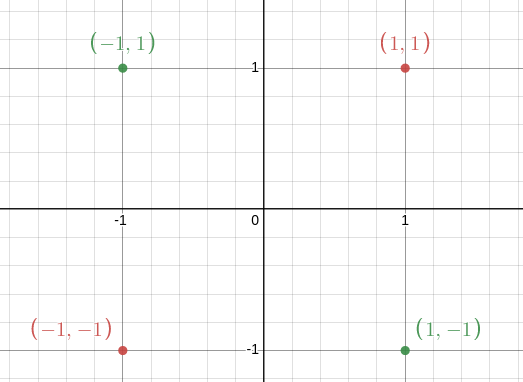
\includegraphics[width=0.5\linewidth]{../outputs/hw1-q3-a.png}
            \caption{Space of $f(x)$ for $D=2, A=-1, B=1$. Green represents class 1 and red represents class -1.}
            \label{fig:3a:graph}
        \end{figure}

        For this example, we can see that the data is not linearly separable, since it is equivalent to the XOR problem which is also not linearly separable. For this reason, we can conclude we cannot use a single perceptron to classify this data.

    \item \textbf{1. b)}
        \begin{equation*}
            f(x) =
            \begin{cases}
                1 & \text{if } \sum_{i=1}^{D} x_i \in [A, B] \\
                -1 & \text{otherwise}
            \end{cases}
        \end{equation*}
        \begin{equation*}
            f(x) =
            \begin{cases}
                1 & \text{if } A \leq \sum_{i=1}^{D} x_i \text{ and } \sum_{i=1}^{D} x_i \leq B \\
                -1 & \text{otherwise}
            \end{cases}
        \end{equation*}

        Let $ S = \sum_{i=1}^{D} x_i $, then:

        \begin{equation*}
            f(x) =
            \begin{cases}
                1 & \text{if } A \leq S \text{ and } S \leq B \\
                -1 & \text{otherwise}
            \end{cases}
        \end{equation*}

        Since $A,B,S \in \mathbb{Z}$, for this domain, the equation above is equivalent to:

        \begin{equation*}
            f(x) =
            \begin{cases}
                1 & \text{if } A-0.5 \leq S \text{ and } S \leq B+0.5 \\
                -1 & \text{otherwise}
            \end{cases}
        \end{equation*}
        \begin{equation}
            f(x) =
            \begin{cases}
                1 & \text{if } 0 \leq S -A+0.5 \text{ and } 0 \leq -S+B+0.5 \\
                -1 & \text{otherwise}
            \end{cases}
            \label{directly-derived-smallerthans}
        \end{equation}

        For the following:

        \[
            b^{[0]} = \begin{bmatrix}
                -A+0.5 \\
                B+0.5
            \end{bmatrix}
            \hspace{2cm}
            W^{[0]} = \begin{bmatrix}
                1 & \hdots & 1 \\
                -1 & \hdots & -1
            \end{bmatrix}
        \]

        We get that:

        \[
            b^{[0]} + W^{[0]} \cdot \textbf{x} =
            \begin{bmatrix}
                -A+0.5 \\
                B+0.5
            \end{bmatrix}
            +
            \begin{bmatrix}
                1 & \hdots & 1 \\
                -1 & \hdots & -1
            \end{bmatrix}
            \cdot
            \begin{bmatrix}
                x_1 \\
                \vdots \\
                x_D
            \end{bmatrix}
            =
            \begin{bmatrix}
                \sum_{i=1}^{D} x_i  -A + 0.5\\
                -\sum_{i=1}^{D} x_i + B + 0.5
            \end{bmatrix}
            =
            \begin{bmatrix}
                S - A + 0.5\\
                -S + B + 0.5
            \end{bmatrix}
        \]

        This result is quite similar to the conditions where the class is +1, in equation \ref{directly-derived-smallerthans}.

        The next step in the MLP is applying the sign function, which applied to the result above, gives us a similar boolean result to the boolean requirements in equation \ref{directly-derived-smallerthans}, where $true = 1$, and $false = -1$.

        \[
            \text{sign}(b^{[0]} + W^{[0]} \cdot \textbf{x}) =
            \begin{bmatrix}
                S - A + 0.5 \geq 0 \\
                -S + B + 0.5 \geq 0
            \end{bmatrix}
        \]

        From analysing equation \ref{directly-derived-smallerthans}, it should get class +1 when both conditions are true, that is, when the result is $\begin{bmatrix}1\\1\end{bmatrix}$.

            The other possible cases are, by permutation, $\begin{bmatrix}1\\-1\end{bmatrix}$, $\begin{bmatrix}-1\\1\end{bmatrix}$ and $\begin{bmatrix}-1\\-1\end{bmatrix}$. All of these should equate to class -1, since they mean at least one of the original conditions is false. However, case $\begin{bmatrix}-1\\-1\end{bmatrix}$ is impossible:

                \begin{figure}[H]
                    \[
                        \begin{bmatrix}
                            -1\\
                            -1
                        \end{bmatrix}
                        \Leftrightarrow
                        \begin{cases}
                            S - A + 0.5 < 0 \\
                            -S + B + 0.5 < 0
                        \end{cases}
                        \Leftrightarrow
                        \begin{cases}
                            S+0.5 < A \\
                            B < S-0.5
                        \end{cases}
                        \Rightarrow
                        B < A
                    \]
                    \caption*{Impossible. $A \leq B$}
                \end{figure}

        The last weight and bias matrices will be as following:

        \[
            b^{[1]} = \begin{bmatrix}
                -1
            \end{bmatrix}
            \hspace{2cm}
            W^{[1]} = \begin{bmatrix}
                1 & 1
            \end{bmatrix}
        \]

        For the three scenarios, this will output what we want:

        \[
            b^{[1]}+W^{[1]}\cdot
            \begin{bmatrix}
                1 \\
                1
            \end{bmatrix}
            =
            2 - 1 = 1
        \]
        \[
            b^{[1]}+W^{[1]}\cdot
            \begin{bmatrix}
                -1 \\
                1
            \end{bmatrix}
            =
            0 - 1 = -1
        \]
        \[
            b^{[1]}+W^{[1]}\cdot
            \begin{bmatrix}
                1 \\
                -1
            \end{bmatrix}
            =
            0 - 1 = -1
        \]

        Given the codomain of $\{-1,1\}$, the final activation function, which is $sign(z)$, will not change the result, and will output directly the correct class.

        The limits can be demonstrably proven to be robust. For this problem, adding an infinitesimal vector to the input vector, will only effect the $\sum_{i=1}^{D} x_i$. These infinitesimal vectors will result in a $S^{'}$, which is either infinitesimally bigger or smaller or equal than $S$, which are $S^{+}$, $S^{-}$, respectively. Let $S-A$ and $-S+B$ be $T$ and $U$, respectively, which as a subtraction between integers, are also integers.

        \[
            \lim_{S^{'}\to S}  h_0(z_0) = 
            \begin{bmatrix}
                S^{'} - A + 0.5 \geq 0  \\
            -S^{'} + B + 0.5 \geq 0
            \end{bmatrix}
            = \lim_{T^{'}\to T \text{ and } U^{'}\to U}  h_0(z_0)
            \begin{bmatrix}
                T^{'} \geq - 0.5 \\
                U^{'} \geq - 0.5
            \end{bmatrix}
        \]

        Since $T,U$ are both integers, this inequality cannot flip with infinitesimal changes. As such, infinitesimal changes to S, in both directions, are equivalent to S.

    \item \textbf{1. c)} For ReLU, it is similar, and we can share work up from the equation \ref{directly-derived-smallerthans}:
        \[
            f(x) =
            \begin{cases}
                1 & \text{if } 0 \leq S -A+0.5 \text{ and } 0 \leq -S+B+0.5 \\
                -1 & \text{otherwise}
            \end{cases}
        \]
        \begin{equation}
            f(x) =
            \begin{cases}
                1 & \text{if } 0 \geq -(S-A+0.5) \text{ and } 0 \geq -(-S+B+0.5) \\
                -1 & \text{otherwise}
            \end{cases}
            \label{directly-derived-greaterthans}
\end{equation}



        Considering the following weight and bias matrices:

        \[
            b^{[0]} = \begin{bmatrix}
                A-0.5 \\
                -B-0.5
            \end{bmatrix}
            \hspace{2cm}
            W^{[0]} = \begin{bmatrix}
                -1 & \hdots & -1 \\
                1 & \hdots & 1
            \end{bmatrix}
        \]

        We get that:

        \[
            b^{[0]} + W^{[0]} \cdot \textbf{x} =
            \begin{bmatrix}
                A-0.5 \\
                -B-0.5
            \end{bmatrix}
            +
            \begin{bmatrix}
                -1 & \hdots & -1 \\
                1 & \hdots & 1
            \end{bmatrix}
            \cdot
            \begin{bmatrix}
                x_1 \\
                \vdots \\
                x_D
            \end{bmatrix}
            =
            \begin{bmatrix}
                -\sum_{i=1}^{D} x_i  + A - 0.5 \\
                \sum_{i=1}^{D} x_i - B - 0.5
            \end{bmatrix}
            =
            \begin{bmatrix}
                - S + A - 0.5\\
                S -B - 0.5
            \end{bmatrix}
            =
        \]
        \begin{equation}
        =
            \begin{bmatrix}
                - (S - A + 0.5)\\
                - (-S + B + 0.5)
                \end{bmatrix}
                \label{z1-relu}
        \end{equation}

        The result are the same conditions present in equation \ref{directly-derived-greaterthans}, but in this case, class +1 requires these values to be smaller than or equal to 0.

        The next step in the MLP is applying the activation function, which will now be ReLU. Applied to the result above:

        \[
            ReLU(
            \begin{bmatrix}
                - (S - A + 0.5)\\
                - (-S + B + 0.5)
            \end{bmatrix}
            ) =
            \begin{bmatrix}
                x \in \mathbb{R}_{\geq 0} \\
                x \in \mathbb{R}_{\geq 0} \\
            \end{bmatrix}
        \]

        From analysing equation \ref{directly-derived-greaterthans}, it should get class +1 when both conditions are true, that is, when the values in equation \ref{z1-relu} are smaller or equal to zero, and false when bigger than zero. Applying $ReLU$ will convert negative numbers, and zero, to 0, and keep positive values as they are. This means that $x = 0 \Leftrightarrow true$ and $x \in \mathbb{R}_{+} \Leftrightarrow false$. As such, class $+1$ corresponds to both conditions being, true, that is, when this result matrix equals $\begin{bmatrix}0\\0\end{bmatrix}$.

            \newcommand{\rmais}{\mathbb{R}_{+}}
            The other possible cases are, by permutation, $\begin{bmatrix}0\\x\in\rmais\end{bmatrix}$, $\begin{bmatrix}x\in\rmais\\0\end{bmatrix}$ and $\begin{bmatrix}x\in\rmais\\x\in\rmais\end{bmatrix}$. All of these should equate to class -1, since they mean at least one of the original conditions is false. However, like in the previous exercise, case $\begin{bmatrix}x\in\rmais\\x\in\rmais\end{bmatrix}$ is impossible:

                \begin{figure}[H]
                    \[
                        \begin{bmatrix}
                        x\in\rmais\\
                        x\in\rmais
                    \end{bmatrix}
                    \Leftrightarrow
                        \begin{cases}
                            -(S-A+0.5) > 0 \\
                            -(-S + B + 0.5) > 0
                        \end{cases}
                        \Leftrightarrow
                        \begin{cases}
                            S+0.5 < A \\
                            B < S-0.5
                        \end{cases}
                        \Rightarrow
                        B < A
                    \]
                    \caption*{Impossible. $A \leq B$}
                \end{figure}

        The last weight and bias matrices will be as following:

        \[
            b^{[1]} = \begin{bmatrix}
                0
            \end{bmatrix}
            \hspace{2cm}
            W^{[1]} = \begin{bmatrix}
                -1 & -1
            \end{bmatrix}
        \]

        For the three scenarios, this will output what we want:

        \[
            b^{[1]}+W^{[1]}\cdot
            \begin{bmatrix}
                0 \\
                0
            \end{bmatrix}
            =
            -0 -0 + 0 = 0
        \]
        \[
            b^{[1]}+W^{[1]}\cdot\begin{bmatrix}x\in\rmais\\0\end{bmatrix}
            =
            - x - 0 + 0 = -x
        \]
        \[
            b^{[1]}+W^{[1]}\cdot\begin{bmatrix}0\\x\in\rmais\end{bmatrix}
            =
            - 0 - x + 0 = -x
        \]

        Finally, by applying the sign function, that is, our output activation, we will get:
        \[
            sign(0) = 1
        \]
        \[
            sign(-x) = -1
        \]
        \[
            sign(-x) = -1
        \]

        Which are the correct results for the three possible scenarios.

        Like above, the limits can be demonstrably proven to be robust. For this problem, adding an infinitesimal vector to the input vector, will only effect the $\sum_{i=1}^{D} x_i$. These infinitesimal vectors will result in a $S^{'}$, which is either infinitesimally bigger or smaller or equal than $S$, which are $S^{+}$, $S^{-}$, respectively. Let $-S+A$ and $S-B$ be $T$ and $U$, respectively, which as a subtraction between integers, are also integers.

        \[
            \lim_{S^{'}\to S}  h_0(z_0) = 
            ReLU(
            \begin{bmatrix}
                - (S^{'} - A + 0.5) \\
                -(-S^{'} + B + 0.5) 
            \end{bmatrix}
            )
            = \lim_{T^{'}\to T \text{ and } U^{'}\to U}  h_0(z_0) =
            ReLU(
            \begin{bmatrix}
                T^{'} - 0.5 \\
                U^{'} - 0.5
            \end{bmatrix}
            )
        \]

        Since $T,U$ are both integers, infinitesimal changes will not change the behaviour of the ReLU, which is converting negative values to 0, and keeping positive values unchanged. Infinitesimal changes will have no effect in changing the activation of the ReLU expression as a whole, since its decimal part is .5 . As such, the operation does not change meaning when approaching from different directions of $S$, and we can conclude that infinitesimal changes to $S$ are equivalent to $S$.

    \end{itemize}

\end{document}
